\documentclass{ximera}

\begin{document}
	\author{Stitz-Zeager}
	\xmtitle{Exercises}


\mfpicnumber{1}
\opengraphsfile{RationalIneq}

\setcounter{footnote}{0}

\label{RationalIneq}

In this section, we solve equations and inequalities involving rational functions and explore associated application problems. Our first example showcases the critical difference in procedure between solving equations and inequalities.

\begin{example} \label{rationalinequalityex}  $~$

\begin{multicols}{2}
\begin{enumerate}

\item  Solve $\dfrac{x^3-2x+1}{x-1} = \dfrac{1}{2}x-1$.

\item  Solve $\dfrac{x^3-2x+1}{x-1} \geq \dfrac{1}{2}x-1$.

\setcounter{HW}{\value{enumi}}
\end{enumerate}
\end{multicols}

\begin{enumerate}
\setcounter{enumi}{\value{HW}}

\item  Verify your solutions using a graphing utility.

\end{enumerate}

{ \bf Solution.} 

\begin{enumerate}

\item  To solve the equation, we clear denominators

\[ \begin{array}{rclr}

\dfrac{x^3-2x+1}{x-1} & = & \dfrac{1}{2}x-1 & \\ [10pt]

\left(\dfrac{x^3-2x+1}{x-1}\right) \cdot 2(x-1) & = & \left( \dfrac{1}{2}x-1 \right) \cdot 2(x-1) & \\ [10pt]

2x^3 - 4x + 2 & = & x^2-3x+2 & \text{expand} \\

2x^3 -x^2 - x & = & 0 & \\

x(2x+1)(x-1) & = & 0 & \text{factor}\\

x & = & -\frac{1}{2}, \, 0, \, 1 & \\


\end{array}\]

Since we cleared denominators, we need to check for extraneous solutions.  Sure enough, we see that $x=1$ does not satisfy the original equation, so  our only solutions are $x=-\frac{1}{2}$ and $x=0$.

\item  To solve the inequality, it may be tempting to begin as we did with the equation $-$ namely by multiplying both sides by the quantity $(x-1)$.  The problem is that, depending on $x$, $(x-1)$ may be positive (which doesn't affect the inequality) or $(x-1)$ could be negative (which would reverse the inequality).  Instead of working by cases, we collect all of the terms on one side of the inequality with $0$ on the other and make a sign diagram using the technique given on page \pageref{rationalsigndiagram} in Section \ref{RationalGraphs}.

\[ \begin{array}{rclr}

\dfrac{x^3-2x+1}{x-1} & \geq & \dfrac{1}{2}x-1 & \\ [10pt]

\dfrac{x^3-2x+1}{x-1}  - \dfrac{1}{2} x + 1& \geq & 0& \\ [10pt]

\dfrac{2 \left(x^3-2x+1\right)}{2(x-1)}  - \dfrac{x(x-1)}{2(x-1)} + \dfrac{2(x-1)}{2(x-1)}& \geq & 0&\text{get a common denominator} \\ [10pt]

\dfrac{2\left(x^3-2x+1\right)-x(x-1)+2(x-1)}{2(x-1)} & \geq & 0 & \\ [10pt]

\dfrac{2x^3-x^2-x}{2x-2} & \geq & 0 & \text{expand} \\

\end{array} \]

Viewing the left hand side as a rational function $r(x)$ we make a sign diagram.  The only value excluded from the domain of $r$ is $x=1$ which is the solution to $2x-2=0$.  The zeros of $r$ are the solutions to $2x^3-x^2-x=0$, which we have already found to be $x=0$, $x=-\frac{1}{2}$ and $x=1$, the latter was discounted as a zero because it is not in the domain.  Choosing test values in each test interval, we construct the sign diagram below. 

\begin{center}

\begin{mfpic}[10]{-6}{6}{-2}{2}
\arrow \reverse \arrow \polyline{(-6,0),(6,0)}
\xmarks{-3,0,3}
\tlpointsep{6pt}
\axislabels {x}{{$-\frac{1}{2} \hspace{7pt}$ } -3, {$0$} 0, {$1$} 3 }
\tlabel[cc](-4.5,1){$(+)$}
\tlabel[cc](-3,1){$0$}
\tlabel[cc](-1.5,1){$(-)$}
\tlabel[cc](0,1){$0$}
\tlabel[cc](1.5,1){$(+)$}
\tlabel[cc](3,1){\textinterrobang}
\tlabel[cc](4.5,1){$(+)$}
\end{mfpic} 

\end{center}

We are interested in where $r(x) \geq 0$.  We see  $r(x) > 0$, or $(+)$, on the intervals $\left(-\infty, -\frac{1}{2}\right)$, $(0,1)$ and $(1, \infty)$.  We know $r(x) = 0$ when  $x = -\frac{1}{2}$ and $x = 0$.   Hence, $r(x) \geq 0$ on  $\left( - \infty, -\frac{1}{2} \right] \cup [0,1) \cup (1, \infty)$.

\item  To check our answers graphically,  let $f(x) = \frac{x^3-2x+1}{x-1}$ and $g(x) = \frac{1}{2} x -1$. The solutions to $f(x)=g(x)$ are the $x$-coordinates of the points where the graphs of $y=f(x)$ and $y=g(x)$ intersect.  We graph both $f$ and $g$ below (the graph of $g$ is the line and is slightly lighter in color.) We find only two intersection points, $(-0.5, -1.25)$ and $(0,-1)$ which correspond to our solutions $x = -\frac{1}{2}$ and $x = 0$.   The solution to $f(x) \geq g(x)$ represents not only where the graphs meet, but the intervals over which the graph of $y=f(x)$ is above ($>$) the graph of $g(x)$.  From the graph, this \textit{appears} to happen on on $\left( - \infty, -\frac{1}{2} \right] \cup [0, \infty)$ which \textit{almost} matches the answer we found analytically.  We have to remember that $f$ is not defined at $x=1$,  so it cannot be included in our solution.\footnote{We invite the reader to show there is a hole in the graph of $y = f(x)$ at $(1,1)$.}


% https://www.desmos.com/calculator/qrwiqyv2bk
\begin{center} 
\desmos{qrwiqyv2bk}{800}{600} 
\end{center}

\end{enumerate}
\end{example}  

The important take-away from Example \ref{rationalinequalityex} is not to clear fractions when working with an inequality unless you know for certain the sign of the denominators. We offer another example.

\begin{example} \label{morerationalineq} Solve:  $2t (3t-2)^{-1} \leq 3t^2 (3t-2)^{-2}$. Check your answer using a graphing utility.


{\bf Solution.} We begin by rewriting the terns with negative exponents as fractions and gathering all nonzero terms to one side of the inequality:

\[ \begin{array}{rclr}

2t (3t-2)^{-1} &  \leq & 3t^2 (3t-2)^{-2} & \\ [10pt]

\dfrac{2t}{3t-2} & \leq & \dfrac{3t^2}{(3t-2)^2} & \\ [10pt]


\dfrac{2t}{3t-2}  - \dfrac{3t^2}{(3t-2)^2}  & \leq & 0 &  \\ [10pt]

\dfrac{2t(3t-2)}{(3t-2)^2}  - \dfrac{3t^2}{(3t-2)^2}  & \leq & 0  & \text{get a common denominator} \\ [10pt]

\dfrac{2t(3t-2) - 3t^2}{(3t-2)^2}  & \leq & 0  &\\ [10pt]

\dfrac{3t^2-4t}{(3t-2)^2}  & \leq & 0  & \text{expand} \\ [10pt]

\end{array} \]

We define $r(t) = \frac{3t^2-4t}{(3t-2)^2}$ and set about constructing a sign diagram for $r$.  Solving  $(3t-2)^2 = 0$ gives $t = \frac{2}{3}$, our sole excluded value.  To find the zeros of $r$, we set $r(t) = \frac{3t^2-4t}{(3t-2)^2} = 0$ and solve $3t^2-4t = 0$.  Factoring gives $t(3t-4) = 0$ so our solutions are $t = 0$ and $t = \frac{4}{3}$. After choosing test values, we  get the sign diagram below on the left.   Since we are looking for where $r(t) \leq 0$, we are looking for where $r(t)$ is $(-)$ or $r(t) = 0$. Hence,  our final answer is $\left[0, \frac{2}{3} \right) \cup \left(\frac{2}{3}, \frac{4}{3} \right]$.  Below on the right,  we graph $f(t) = 2t(3t-1)^{-1}$ (the darker curve),   $g(t) = 3t^2(3t-2)^{-2}$, and  vertical asymptote $x = \frac{2}{3}$, the dashed line.  Sure enough, the graph of $f$ intersects the graph of $g$ when $t = 0$ and $t = \frac{4}{3}$.  Moreover, the graph of $f$ is below the graph of $g$ everywhere they are defined between these values, in accordance with our algebraic solution.



\begin{mfpic}[10]{-6}{6}{-2}{2}
\arrow \reverse \arrow \polyline{(-6,0),(6,0)}
\xmarks{-3,0,3}
\tlpointsep{6pt}
\axislabels {x}{{$0 \hspace{7pt}$ } -3, {$\frac{2}{3}$} 0, {$\frac{4}{3}$} 3 }
\tlabel[cc](-4.5,1){$(+)$}
\tlabel[cc](-3,1){$0$}
\tlabel[cc](-1.5,1){$(-)$}
\tlabel[cc](0,1){\textinterrobang}
\tlabel[cc](1.5,1){$(-)$}
\tlabel[cc](3,1){$0$}
\tlabel[cc](4.5,1){$(+)$}
\end{mfpic} 



% https://www.desmos.com/calculator/mngh4jcrvl
\begin{center} 
\desmos{mngh4jcrvl}{800}{600} 
\end{center}

\end{example}

One thing to note about Example \ref{morerationalineq} is that the quantity $(3t-2)^2 \geq 0$ for all values of $t$.  Hence, as long as we remember $t = \frac{2}{3}$ is excluded from consideration, we could actually multiply both sides of the inequality in  Example \ref{morerationalineq} by $(3t-2)^2$ to obtain $2t(3t-2) \leq 3t^2$.  We could then solve this (slightly easier) inequality using the methods of Section \ref{QuadraticFunctions} as long as we remember to exclude $t = \frac{2}{3}$  from our solution. Once again, the more you \textit{understand}, the less you have to \textit{memorize}.  If you know the `\textit{why}' behind an algorithm instead of just the `\textit{how},' you will know when you can short-cut it.

Our next example is an application of average cost.  Recall from Definition \ref{averagecostprofit} if $C(x)$ represents the cost to make $x$ items then the average cost per item  is given by $\overline{C}(x) = \frac{C(x)}{x}$, for $x>0$. 

\begin{example} \label{averagecostapp} Recall from Example \ref {PortaBoyCost} that the cost,  $C(x)$, in dollars, to produce $x$ PortaBoy game systems for a local retailer is $C(x) = 80x + 150$, $x \geq 0$.

\begin{enumerate}

\item  Find an expression for the average cost function, $\overline{C}(x)$. 

\item  \label{costlessthan} Solve $\overline{C}(x) < 100$ and interpret.

\item  Find and interpret $\ds{\lim_{x \rightarrow \infty} \overline{C}(x)}$.


\end{enumerate}

{\bf Solution.}

\begin{enumerate}

\item  From $\overline{C}(x) = \frac{C(x)}{x}$, we obtain $\overline{C}(x) = \frac{80x+150}{x}$.  The domain of $C$ is $x \geq 0$, but since $x=0$ causes problems for $\overline{C}(x)$, we get our domain to be $x>0$, or $(0, \infty)$.

\item  Solving $\overline{C}(x) < 100$ means we solve $\frac{80x+150}{x} < 100$.  We proceed as in the previous example.

\[ \begin{array}{rclr}

\dfrac{80x+150}{x} & < & 100 & \\ [10pt]

\dfrac{80x+150}{x} - 100 & < & 0 & \\ [10pt]

\dfrac{80x + 150 - 100x}{x} & < & 0 & \text{common denominator} \\ [10pt]

\dfrac{150 - 20x}{x} & < & 0 & \\

\end{array} \]

If we take the left hand side to be a rational function $r(x)$, we need to keep in mind that the applied domain of the problem is $x > 0$.  This means we consider only the positive half of the number line for our sign diagram.  On $(0, \infty)$, $r$ is defined everywhere so we need only look for zeros of $r$.  Setting $r(x)=0$ gives $150-20x =0$, so that $x = \frac{15}{2}= 7.5$.  The test intervals on our domain are $(0, 7.5)$ and $(7.5, \infty)$.  We find $r(x) < 0$ on $(7.5, \infty)$.  

\begin{center}

\begin{mfpic}[10]{0}{8}{-2}{2}
\arrow \polyline{(0,0), (8,0)}
\xmarks{0,4}
\tlabel[cc](0,-1){$0$}
\tlabel[cc](0,1){\textinterrobang}
\tlabel[cc](4,-1){$7.5$}
\tlabel[cc](2,1){$(+)$}
\tlabel[cc](4,1){$0$}
\tlabel[cc](6,1){$(-)$}
\end{mfpic}

\end{center}

In the context of the problem, $x$ represents the number of PortaBoy games systems produced and $\overline{C}(x)$ is the average cost to produce each system.  Solving $\overline{C}(x) < 100$ means we are trying to find how many systems we need to produce so that the average cost is less than $\$100$ per system.  Our solution, $(7.5, \infty)$ tells us that we need to produce more than $7.5$ systems to achieve this.  Since it doesn't make sense to produce half a system, our final answer is $[8, \infty)$.

\item  To find $\ds{\lim_{x \rightarrow \infty} \overline{C}(x)}$, we note that we can rewrite $\overline{C}(x) = \frac{80x+150}{x}  =  80 + \frac{150}{x}$.    As $x \rightarrow \infty$, note that $\frac{150}{x} \rightarrow 0$ so $\ds{\lim_{x \rightarrow \infty} \overline{C}(x) = 80 + 0 = 80}$.   Thus the average cost per system is getting closer to $\$ 80$ per system. Since  $\frac{150}{x} > 0$ for all $x>0$,  we have that  $\overline{C}(x) > 80$ for all $x > 0$.  This means that the average cost per system is always greater than $\$ 80$ per system, but the average cost is approaching this amount as more and more systems are produced.  Looking back at Example \ref{PortaBoyCost}, we realize $\$ 80$ is the variable cost per system $-$ the cost per system above and beyond the fixed initial cost of $\$150$.  Another way to interpret our answer is that `infinitely' many systems would need to be produced to effectively `zero out'  the fixed cost. \qed



\end{enumerate}

\end{example}

Note that number \ref{costlessthan} in Example \ref{averagecostapp} is another opportunity to short-cut the standard algorithm and obtain the solution more quickly if we take stock of the situation.  Since the applied domain is $x>0$, we can multiply through the inequality $\frac{80x+150}{x}  <  100$ by $x$ without worrying about changing the sense of the inequality.  This reduces the problem to  $80x+150 < 100x$, a basic linear inequality whose solution is readily seen to be $x > 7.5$.   It is absolutely critical here that $x>0$. Indeed, any time you decide to multiply an inequality by a variable expression, it is necessary to justify why the inequality is preserved.  Our next example is another classic `box with no top' problem.  The reader is encouraged to compare and contrast this problem with  Example \ref{boxnotopex} in Section \ref{GraphsofPolynomials}.

\begin{example}  \label{boxnotopfixedvolume} A box with a square base and no top is to be constructed so that it has a volume of $1000$ cubic centimeters.  Let $x$ denote the width of the box, in centimeters as seen below.

\begin{center}

\begin{mfpic}[15]{-2}{8}{-2}{4}
\polyline{(0,0),(0,1)}
\polyline{(4,0), (4,1)}
\polyline{(0,1),(2,3)}
\polyline{(4,1),(6,3)}
\polyline{(0,0),(4,0)}
\polyline{(0,1),(4,1)}
\polyline{(2,3),(6,3)}
\polyline{(4,0),(6,2)}
\polyline{(6,3),(6,2)}
\polyline{(2,3),(2,2)}
\polyline{(2,2),(5,2)}
\dotted \polyline{(5,2),(6,2)}
\polyline{(2,2),(1,1)}
\dotted \polyline{(1,1),(0,0)}
\arrow \reverse \arrow \polyline{(0,-0.5),(4,-0.5)}
\tlabel[cc](2,-1.5){\scriptsize width, $x$}
\arrow \reverse \arrow \polyline{(-0.5,0), (-0.5,1)}
\tlabel[cc](-1.5,0.5){\scriptsize height}
\arrow \reverse \arrow \polyline{(4.5, -0.25), (6.5,1.75)}
\tlabel[cc](6,0.25){\scriptsize depth}
\end{mfpic}


\end{center}


\begin{enumerate}

\item  Explain why the height of the box (in centimeters) is a function of the width $x$. Call this function $h$ and find an expression for $h(x)$, complete with an appropriate applied domain.

\item  Solve $h(x) \geq x$ and interpret.

\item  Find and interpret $\ds{\lim_{x \rightarrow 0^{+}} h(x)}$ and $\ds{\lim_{x \rightarrow \infty} h(x)}$ .

\item  Express the surface area of the box as a function of $x$, $S(x)$ and state the applied domain.

\item  Use a graphing utility  to approximate (to two decimal places) the dimensions of the box which minimize the surface area.

\end{enumerate}

{ \bf Solution.}

\begin{enumerate}

\item  We are told that the volume of the box is $1000$ cubic centimeters and that $x$ represents the width, in centimeters.  Since $x$ represents a physical dimension of a box, we have that $x>0$.  From geometry, we know $\text{volume} = \text{width} \times \text{height} \times \text{depth}$.  Since the base of the box is a square, the width and the depth are both $x$ centimeters.  Hence,  $1000 = x^2 (\text{height})$. Solving for the height, we get $\text{height} = \frac{1000}{x^2}$.   In other words, for each width $x>0$, we are able to compute \textit{the}\footnote{that is, the one and only one} corresponding height using the formula $\frac{1000}{x^2}$.  Hence, the height is a function of $x$.    Using function notation, we write $h(x) = \frac{1000}{x^2}$.  As mentioned before, our only restriction is $x>0$ so the domain of $h$ is $(0, \infty)$.

% https://www.geogebra.org/classic/zv4shrqn
\begin{center}
\geogebra{zv4shrqn}{800}{600}
\end{center}

\item  To solve $h(x) \geq x$, we proceed as before and collect all nonzero terms on one side of the inequality in order to use a sign diagram.

\[ \begin{array}{rclr}

h(x) & \geq & x & \\ [10pt]

\dfrac{1000}{x^2} & \geq & x & \\ [10pt]

\dfrac{1000}{x^2} - x & \geq & 0 \\ [10pt]

\dfrac{1000-x^3}{x^2} & \geq & 0 & \text{common denominator} \\[10pt]

\end{array} \]

We consider the left hand side of the inequality as our rational function $r(x)$.  We see immediately the only value excluded from the domain of $r$ is $0$, but since our applied domain is $x>0$, we restrict our attention to the interval  $(0, \infty)$.  The sole zero of $r$ comes when $1000-x^3 = 0$,  or when $x=10$.  Choosing test values in the intervals $(0,10)$ and $(10, \infty)$ gives the following:

\begin{center}

\begin{mfpic}[10]{0}{8}{-2}{2}

\arrow \polyline{(0,0), (8,0)}

\xmarks{0,4}

\tlabel[cc](0,-1){$0$}

\tlabel[cc](0,1){\textinterrobang}

\tlabel[cc](2,1){$(+)$}

\tlabel[cc](4,-1){$10$}

\tlabel[cc](4,1){$0$}

\tlabel[cc](6,1){$(-)$}

\end{mfpic}

\end{center}

We see $r(x) > 0$ on $(0,10)$, and since $r(x) = 0$ at $x=10$, our solution is $(0,10]$.  In the context of the problem, $h(x)$ represents the height of the box while $x$ represents the width (and depth) of the box.  Solving $h(x) \geq x$ is tantamount to finding the values of $x$ which result in a box where the height is at least as big as the width (and, in this case, depth.)  Our answer tells us the width of the box can be at most $10$ centimeters for this to happen.\footnote{As with the previous example, knowing $x>0$ means  $x^2>0$ so we can clear denominators right away and solve $x^3 \leq 1000$, or $x \leq 10$.  Coupled with our applied domain, $x>0$, we would arrive at the same solution, $(0, 10]$.}

% https://www.geogebra.org/classic/qdacpjpp
\begin{center}
\geogebra{qdacpjpp}{800}{600}
\end{center}

\item Since $h(x) = \frac{1000}{x^2}$, $\ds{\lim_{x \rightarrow 0^{+}} h(x) = \infty}$.  This means that the smaller the width $x$  (and, in this case, depth), the larger the height $h$ has to be in order to maintain a volume of $1000$ cubic centimeters. On the other hand, $\ds{\lim_{x \rightarrow \infty} h(x) = 0}$, which means that in order to maintain a volume of $1000$ cubic centimeters, the width and depth must get bigger as the height becomes smaller.

\item  Since the box has no top, the surface area can be found by adding the area of each of the sides to the area of the base.  The base is a square of dimensions $x$ by $x$, and each side has dimensions $x$ by $h(x)$.  We get the surface area, $S(x) = x^2+4xh(x)$.  Since $h(x) = \frac{1000}{x^2}$, we have  $S(x) = x^2+4x \left( \frac{1000}{x^2}\right)= x^2 + \frac{4000}{x}$.  The domain of $S$ is the same as $h$, namely $(0, \infty)$, for the same reasons as above.

\item   To graph $y = S(x)$, we create a table of values to help us define a good viewing window.  Doing so, we find a local minim when $x \approx 12.60$.  As far as we can tell,\footnote{without Calculus, that is...} this is the only local extremum, so it is the (absolute) minimum as well. This means that the width and depth of the box should each measure approximately $12.60$ centimeters.  To determine the height, we find $h(12.60) \approx 6.30$, so the height of the box should be approximately $6.30$ centimeters.\footnote{The $y$-coordinate here, $476.22$ means the minimum surface area possible is $476.22$ square centimeters.  Minimizing the surface area minimizes the material required to make the box, therein helping to reduce the cost of the box.}

\begin{center}


\includegraphics[width=4in]{./RationalIneqGraphics/RatIneqEx04.jpg} 


\end{center} 

\end{enumerate}
\qed

\end{example}

Our last example uses regression to verify a very famous scientific law.

\begin{example}  \label{BoyleslawRational} Boyle's Law states that when temperature is held constant, the pressure of a gas is inversely proportional to the volume of the gas.\footnote{For a review of what this means, see Section \ref{AppVariation}.}  According to this \href{http://web.lemoyne.edu/~giunta/classicalcs/boyleverify.html}{\underline{website}} the actual data relating the volume $V$ of a gas and its pressure $P$ used by Boyle and his assistant in 1662 to formulate this law is given below. (NOTE: both pressure and volume here are given in `arbitrary units.')

\[ \begin{array}{|c||c|c|c|c|c|c|c|c|c|c|c|c|c|}  \hline

V & 48 & 46 & 44 & 42 & 40 & 38 & 36 & 34 & 32 & 30 & 28 & 26 & 24  \\ \hline

P & 29.13 & 30.56 & 31.94 & 33.5 & 35.31 & 37 & 39.31 & 41.63 & 44.19 & 47.06 & 50.31 & 54.31 & 58.81  \\ \hline \end{array} \]


\[\begin{array}{|c||c||c|c|c|c|c|c|c|c|c|c|c|c|} \hline

V & 23 & 22 & 21 & 20 & 19 & 18 & 17 & 16 & 15 & 14 & 13 & 12  \\ \hline 

P & 61.31 & 64.06 & 67.06 & 70.69 & 74.13 & 77.88 & 82.75 & 87.88 & 93.06 & 100.44 & 107.81 & 117.56   \\ \hline \end{array} \]

\begin{enumerate}

\item Assuming  $P$ and $V$ are inversely proportional, estimate  the constant of proportionality, $k$.

\item Use a graphing utility to fit a curve of the form $P = \dfrac{k}{V}$ to these data.  

\end{enumerate}
 
{\bf Solution.}

\begin{enumerate}

\item Recall if $P$ and $V$ are inversely proportional, there is a real number $k$ so $PV = k$ for all values of $P$ and $V$.  Multiplying the corresponding $P$ and $V$ values from the data together result in numbers which are consistently approximately $1400$.  This gives us confidence in the claim $P$ and $V$ are inversely proportional and suggests $k \approx 1400$.

\item  We plot the pairs $(V, P)$ and run a regression, the results of which are below.  To our amazement, the graphing utility reports $k \approx 1406.9$ with  $R^2 \approx 1$.  This means the data are a very good fit to the model $P = \frac{k}{V}$, or $PV = k$, hence verifying Boyle's Law for this set of data.

\begin{center}

\includegraphics[width=6in]{./RationalIneqGraphics/BoylesLawEx.jpg} 

\end{center}


\end{enumerate}
\qed

\end{example}

\newpage

\subsection{Exercises}

%% SKIPPED %% \documentclass{ximera}

\begin{document}
	\author{Stitz-Zeager}
	\xmtitle{Exercises for Rational Inequalities}{}

\mfpicnumber{1} \opengraphsfile{ExercisesforRationalIneq} % mfpic settings added 

\begin{question}
(Review of Solving Equations):\footnote{For more review, see Section \ref{AppRatExpEqus}.} 

In Exercises \ref{ratleqnexercisefirst} - \ref{ratleqnexerciselast},  solve the rational equation.  Be sure to check for extraneous solutions.

\begin{problem}\label{ratleqnexercisefirst}
$\dfrac{x}{5x + 4} = 3$ 

\begin{solution}
$x = -\frac{6}{7}$
\end{solution}
\end{problem}

\begin{problem}
$\dfrac{3x - 1}{x^{2} + 1} = 1$ 
\end{problem} 

\begin{problem}
$\dfrac{1}{t + 3} + \dfrac{1}{t - 3} = \dfrac{t^{2} - 3}{t^{2} - 9}$ 

\begin{solution}
$t = -1$
\end{solution}
\end{problem} 

\begin{problem}
$\dfrac{2t + 17}{t + 1} = t + 5$ 
\end{problem}  

\begin{problem}
$\dfrac{z^{2} - 2z + 1}{z^{3} + z^{2} - 2z} = 1$ 

\begin{solution}
No solution
\end{solution}
\end{problem}   

\begin{problem}\label{ratleqnexerciselast}
$\dfrac{4z- z^3}{z^{2} - 9} = 4z$  
\end{problem}  

\end{question}

\begin{question}
In Exercises \ref{ratlineqexercisefirst} - \ref{ratlineqexerciselast}, solve the rational inequality.  Express your answer using interval notation.


\begin{problem}\label{ratlineqexercisefirst}
$\dfrac{1}{x + 2} \geq 0$ 

For what value is the rational function undefined? 

$x = \answer{-2}$

\begin{exercise}
Use test points to determine all intervals which are part of the solution set.

    \begin{selectAll}
    \choice{$(-\infty,-2)$} \choice[correct]{$(-2,\infty)$}
  \end{selectAll}
\end{exercise}
\end{problem} 

\begin{problem}
$\dfrac{5}{x + 2} \geq 1$
\end{problem} 

\begin{problem}
$\dfrac{x}{x^{2} - 1} <  0$

For which values is the rational function undefined? (Give your answers in increasing order.)

For which value is the rational function equal to 0? $x = \answer{0}$

$x = \answer{-1}$, \quad x = $\answer{1}$

\begin{exercise}
Use test points to determine all intervals which are part of the solution set.

    \begin{selectAll}
    \choice[correct]{$(-\infty,-1)$} 
    \choice{$(-1,0)$}
    \choice[correct]{$(0,1)$} 
    \choice{$(1,\infty)$}
  \end{selectAll}
\end{exercise}
\end{problem}  

\begin{problem}
$\dfrac{4t}{t^2+4} \geq 0$
\end{problem}    

\begin{problem}
$\dfrac{2t+6}{t^2+t-6} < 1$

\begin{solution}
$(-\infty, -3) \cup (-3,2) \cup (4, \infty)$
\end{solution}
\end{problem}

\begin{problem}
$\dfrac{5}{t-3} + 9 < \dfrac{20}{t+3}$
\end{problem}

\begin{problem}
$\dfrac{6z+6}{2+z-z^2} \leq z+3$

\begin{solution}
$(-1,0] \cup (2, \infty)$    
\end{solution}
\end{problem}  

\begin{problem}
$\dfrac{6}{z-1} + 1 > \dfrac{1}{z+1}$
\end{problem}  

\begin{problem}
$\dfrac{3z - 1}{z^{2} + 1} \leq 1$

\begin{solution}
$(-\infty, 1] \cup [2, \infty)$
\end{solution}
\end{problem}

\begin{problem}
$(2x+17)(x+1)^{-1} > x + 5$
\end{problem} 

\begin{problem}
$(4x-x^3)(x^{2} - 9)^{-1} \geq 4x$

\begin{solution}
$(-\infty, -3) \cup \left[-2\sqrt{2}, 0\right] \cup \left[2\sqrt{2}, 3\right)$
\end{solution}
\end{problem} 

\begin{problem}
$(x^{2} + 1)^{-1} < 0$
\end{problem}  

\begin{problem}
$(2t-8)(t+1)^{-1} \leq (t^2-8t)(t+1)^{-2}$ 

\begin{solution}
$[-4, -1) \cup (-1,2]$
\end{solution}
\end{problem}  

\begin{problem}
$(t-3)(2t+7)(t^2+7t+6)^{-2} \geq (t^2+7t+6)^{-1}$ % $(-\infty, -6) \cup (-6, -3] \cup [9, \infty)$
\end{problem} 

\begin{problem}
$60z^{-2}+23z^{-1} \geq 7(z-4)^{-1}$

\begin{solution}
$[-3,0) \cup (0,4) \cup [5, \infty)$
\end{solution}
\end{problem} 

\begin{problem}\label{ratlineqexerciselast}
$2z+6(z-1)^{-1} \geq 11 - 8(z+1)^{-1}$
\end{problem}  
\end{question}

\begin{question}
In Exercises \ref{solverationalineqfromgraphfirst} - \ref{solverationalineqfromgraphlast}, use the the graph of the given rational function to  solve the stated inequality.    

\begin{problem}\label{solverationalineqfromgraphfirst}
Solve $f(x) \geq 0$.


\begin{tikzpicture}
  \begin{axis}[
    axis lines=middle,
    xmin=-7, xmax=7,
    ymin=-6, ymax=8,
    xtick={-6,-5,-4,-3,-2,-1,1,5,6},
    xticklabels={$-6$,$-5$,$-4$,$-3$,$-2$,$-1$,$1$,$5$,$6$},
    ytick={-5,-4,-3,-2,-1,1,2,3,4},
    yticklabels={$-5$,$-4$,$-3$,$-2$,$-1$,$1$,$2$,$3$,$4$},
    axis line style={->},
    width=11cm, height=8cm,
    clip=false
  ]
    % Axis labels
    \node at (axis cs:7,-0.5) {\scriptsize $x$};
    \node at (axis cs:0.5,8) {\scriptsize $y$};

    % Horizontal asymptote y=1
    \draw[dashed] (axis cs:-7,1) -- (axis cs:7,1);

    % Vertical asymptote x=0
    \draw[dashed] (axis cs:0,-6) -- (axis cs:0,8);

    % Function y = 1 - 3/x
    \addplot[domain=-7:-0.45, samples=200, thick, ->] {1 - 3/x};
    \addplot[domain=0.45:7, samples=200, thick, ->] {1 - 3/x};

    % Point (3,0)
    \addplot[only marks, mark=*] coordinates {(3,0)};
    \node at (axis cs:3.5,-1) {\scriptsize $(3,0)$};

    % Caption
    \node[below] at (rel axis cs:0.5,0) 
      {\scriptsize $y=f(x)$, asymptotes: $x=0$, $y=1$};
  \end{axis}
\end{tikzpicture}

\begin{solution}
$f(x) \geq 0$ on $(-\infty, 0) \cup [3, \infty)$.
\end{solution}
\end{problem}

\begin{problem}
Solve $f(x) < 1$.


\begin{tikzpicture}
  \begin{axis}[
    axis lines=middle,
    xmin=-7, xmax=7,
    ymin=-6, ymax=8,
    xtick={-6,-5,-4,-3,-2,-1,1,5,6},
    xticklabels={$-6$,$-5$,$-4$,$-3$,$-2$,$-1$,$1$,$5$,$6$},
    ytick={-5,-4,-3,-2,-1,1,2,3,4},
    yticklabels={$-5$,$-4$,$-3$,$-2$,$-1$,$1$,$2$,$3$,$4$},
    axis line style={->},
    width=11cm, height=8cm,
    clip=false
  ]
    % Axis labels
    \node at (axis cs:7,-0.5) {\scriptsize $x$};
    \node at (axis cs:0.5,8) {\scriptsize $y$};

    % Horizontal asymptote y=1
    \draw[dashed] (axis cs:-7,1) -- (axis cs:7,1);

    % Vertical asymptote x=0
    \draw[dashed] (axis cs:0,-6) -- (axis cs:0,8);

    % Function y = 1 - 3/x
    \addplot[domain=-7:-0.45, samples=200, thick, ->] {1 - 3/x};
    \addplot[domain=0.45:7, samples=200, thick, ->] {1 - 3/x};

    % Point (3,0)
    \addplot[only marks, mark=*] coordinates {(3,0)};
    \node at (axis cs:3.5,-1) {\scriptsize $(3,0)$};

    % Caption
    \node[below] at (rel axis cs:0.5,0) 
      {\scriptsize $y=f(x)$, asymptotes: $x=0$, $y=1$};
  \end{axis}
\end{tikzpicture}

\end{problem} 

\begin{problem}
Solve $g(t) \geq  -1 $. 

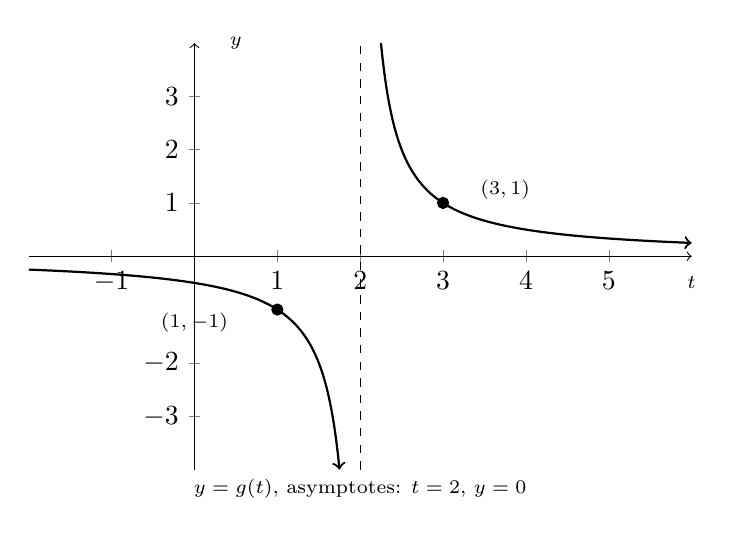
\begin{tikzpicture}
  \begin{axis}[
    axis lines=middle,
    xmin=-2, xmax=6,
    ymin=-4, ymax=4,
    xtick={-1,1,2,3,4,5},
    xticklabels={$-1$,$1$,$2$,$3$,$4$,$5$},
    ytick={-3,-2,1,2,3},
    yticklabels={$-3$,$-2$,$1$,$2$,$3$},
    axis line style={->},
    width=10cm, height=7cm,
    clip=false
  ]
    % Axis labels
    \node at (axis cs:6,-0.5) {\scriptsize $t$};
    \node at (axis cs:0.5,4) {\scriptsize $y$};

    % Vertical asymptote t=2
    \draw[dashed] (axis cs:2,-4) -- (axis cs:2,4);

    % Horizontal asymptote y=0
    \draw[dashed] (axis cs:-2,0) -- (axis cs:6,0);

    % Function y = 1/(x-2)
    \addplot[domain=-2:1.75, samples=200, thick, ->] {1/(x-2)};
    \addplot[domain=2.25:6, samples=200, thick, ->] {1/(x-2)};

    % Solid points
    \addplot[only marks, mark=*] coordinates {(1,-1) (3,1)};
    \node at (axis cs:3.75,1.25) {\scriptsize $(3,1)$};
    \node at (axis cs:0,-1.25) {\scriptsize $(1,-1)$};

    % Caption
    \node[below] at (rel axis cs:0.5,0) 
      {\scriptsize $y=g(t)$, asymptotes: $t=2$, $y=0$};
  \end{axis}
\end{tikzpicture}

\begin{solution}
$g(t) \geq -1$ on $(-\infty, 1] \cup (2, \infty)$.
\end{solution}
\end{problem}   

\begin{problem}
Solve $-1 \leq g(t)  < 1$. 

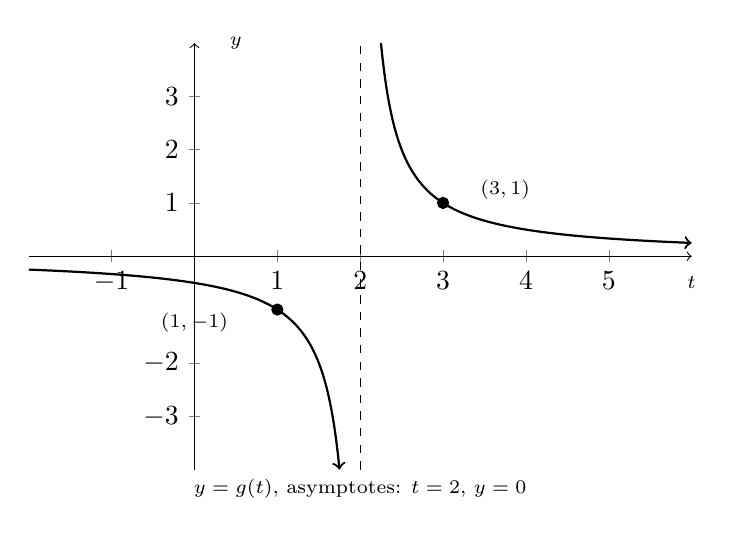
\begin{tikzpicture}
  \begin{axis}[
    axis lines=middle,
    xmin=-2, xmax=6,
    ymin=-4, ymax=4,
    xtick={-1,1,2,3,4,5},
    xticklabels={$-1$,$1$,$2$,$3$,$4$,$5$},
    ytick={-3,-2,1,2,3},
    yticklabels={$-3$,$-2$,$1$,$2$,$3$},
    axis line style={->},
    width=10cm, height=7cm,
    clip=false
  ]
    % Axis labels
    \node at (axis cs:6,-0.5) {\scriptsize $t$};
    \node at (axis cs:0.5,4) {\scriptsize $y$};

    % Vertical asymptote t=2
    \draw[dashed] (axis cs:2,-4) -- (axis cs:2,4);

    % Horizontal asymptote y=0
    \draw[dashed] (axis cs:-2,0) -- (axis cs:6,0);

    % Function y = 1/(x-2)
    \addplot[domain=-2:1.75, samples=200, thick, ->] {1/(x-2)};
    \addplot[domain=2.25:6, samples=200, thick, ->] {1/(x-2)};

    % Solid points
    \addplot[only marks, mark=*] coordinates {(1,-1) (3,1)};
    \node at (axis cs:3.75,1.25) {\scriptsize $(3,1)$};
    \node at (axis cs:0,-1.25) {\scriptsize $(1,-1)$};

    % Caption
    \node[below] at (rel axis cs:0.5,0) 
      {\scriptsize $y=g(t)$, asymptotes: $t=2$, $y=0$};
  \end{axis}
\end{tikzpicture}
\end{problem} 

\begin{problem}
Solve $r(z) \leq 1$ 

\begin{tikzpicture}
  \begin{axis}[
    axis lines=middle,
    xmin=-5, xmax=5,
    ymin=-1, ymax=6,
    xtick={-4,-3,-2,-1,1,2,3,4},
    xticklabels={$-4$,$-3$,$-2$,$-1$,$1$,$2$,$3$,$4$},
    ytick={1,2,3,4,5},
    yticklabels={$1$,$2$,$3$,$4$,$5$},
    axis line style={->},
    width=11cm, height=8cm,
    clip=false
  ]
    % Axis labels
    \node at (axis cs:5,-0.5) {\scriptsize $z$};
    \node at (axis cs:0.5,6) {\scriptsize $y$};

    % Vertical asymptote z=0
    \draw[dashed] (axis cs:0,-1) -- (axis cs:0,6);

    % Horizontal asymptote y=0
    \draw[dashed] (axis cs:-5,0) -- (axis cs:5,0);

    % Function y = 1/x^2
    \addplot[domain=-5:-0.42, samples=200, thick, ->] {1/(x^2)};
    \addplot[domain=0.42:5, samples=200, thick, ->] {1/(x^2)};

    % Solid point (-1,1)
    \addplot[only marks, mark=*] coordinates {(-1,1)};
    \node at (axis cs:-2.5,1) {\scriptsize $(-1,1)$};

    % Hole at (1,1)
    \addplot[only marks, mark=o, mark size=2pt, thick] coordinates {(1,1)};
    \node at (axis cs:3,1) {\scriptsize hole at $(1,1)$};

    % Caption
    \node[below] at (rel axis cs:0.5,0) 
      {\scriptsize $y=r(z)$, asymptotes: $z=0$, $y=0$};
  \end{axis}
\end{tikzpicture}


\end{problem} 

\begin{problem}\label{solverationalineqfromgraphlast} Solve $r(z) > 0$.


\begin{tikzpicture}
  \begin{axis}[
    axis lines=middle,
    xmin=-5, xmax=5,
    ymin=-1, ymax=6,
    xtick={-4,-3,-2,-1,1,2,3,4},
    xticklabels={$-4$,$-3$,$-2$,$-1$,$1$,$2$,$3$,$4$},
    ytick={1,2,3,4,5},
    yticklabels={$1$,$2$,$3$,$4$,$5$},
    axis line style={->},
    width=11cm, height=8cm,
    clip=false
  ]
    % Axis labels
    \node at (axis cs:5,-0.5) {\scriptsize $z$};
    \node at (axis cs:0.5,6) {\scriptsize $y$};

    % Vertical asymptote z=0
    \draw[dashed] (axis cs:0,-1) -- (axis cs:0,6);

    % Horizontal asymptote y=0
    \draw[dashed] (axis cs:-5,0) -- (axis cs:5,0);

    % Function y = 1/x^2
    \addplot[domain=-5:-0.42, samples=200, thick, ->] {1/(x^2)};
    \addplot[domain=0.42:5, samples=200, thick, ->] {1/(x^2)};

    % Solid point (-1,1)
    \addplot[only marks, mark=*] coordinates {(-1,1)};
    \node at (axis cs:-2.5,1) {\scriptsize $(-1,1)$};

    % Hole at (1,1)
    \addplot[only marks, mark=o, mark size=2pt, thick] coordinates {(1,1)};
    \node at (axis cs:3,1) {\scriptsize hole at $(1,1)$};

    % Caption
    \node[below] at (rel axis cs:0.5,0) 
      {\scriptsize $y=r(z)$, asymptotes: $z=0$, $y=0$};
  \end{axis}
\end{tikzpicture}


\end{problem} 

\end{question}


\begin{problem}
In Exercise \ref{newportaboycost} in Section \ref{GraphsofPolynomials},  the function $C(x) = .03x^{3} - 4.5x^{2} + 225x + 250$, for $x \geq 0$ was used to model the cost (in dollars) to produce $x$ PortaBoy game systems. Using this cost function, find the number of PortaBoys which should be produced to minimize the average cost $\overline{C}$.  Round your answer to the nearest number of systems.     
\end{problem}  

\begin{problem}
Suppose we are in the same situation as Example \ref{boxnotopfixedvolume}.  If the volume of the box is to be $500$ cubic centimeters, use a graphing utility to find the dimensions of the box which minimize the surface area.  What is the minimum surface area?  Round your answers to two decimal places.
\end{problem} 

\begin{problem}
The box for the new Sasquatch-themed cereal, `Crypt-Os', is to have a volume of $140$ cubic inches.  For aesthetic reasons, the height of the box needs to be $1.62$ times the width of the base of the box.\footnote{1.62 is a crude approximation of the so-called `Golden Ratio' $\phi = \frac{1 + \sqrt{5}}{2}$.}  Find the dimensions of the box which will minimize the surface area of the box.  What is the minimum surface area?  Round your answers to two decimal places.   
\end{problem}   

\begin{problem}\label{fixedareaminperimetergarden} 
Sally is Skippy's neighbor from Exercise \ref{fixedperimetermaxareagarden} in Section \ref{QuadraticFunctions}.   Sally also wants to plant a vegetable garden along the side of her home.  She doesn't have any fencing, but wants to keep the size of the garden to 100 square feet.  What are the dimensions of the garden which will minimize the amount of fencing she needs to buy?  What is the minimum amount of fencing she needs to buy? Round your answers to the nearest foot. (Note:  Since one side of the garden will border the house, Sally doesn't need fencing along that side.)
\end{problem}

\begin{problem}
Another Classic Problem: A can is made in the shape of a right circular cylinder and is to hold one pint. (For dry goods, one pint is equal to $33.6$ cubic inches.)\footnote{According to \href{http://dictionary.reference.com/browse/pint}{\underline{www.dictionary.com}}, there are different values given for this conversion. We use $33.6 \text{in}^{3}$ for this problem.}  

\begin{enumerate}

\item Find an expression for the volume $V$ of the can in terms of the height $h$ and the base radius $r$.
\item Find an expression for the surface area $S$ of the can in terms of the height $h$ and the base radius $r$.  (Hint: The top and bottom of the can are circles of radius $r$ and the side of the can is really just a rectangle that has been bent into a cylinder.)
\item Using the fact that $V = 33.6$, write $S$ as a function of $r$ and state its applied domain.
\item Use your graphing calculator to find the dimensions of the can which has minimal surface area.

\end{enumerate}
\end{problem}

\begin{problem}
A right cylindrical drum is to hold 7.35 cubic feet of liquid.  Find the dimensions (radius of the base and height) of the drum which would minimize the surface area.  What is the minimum surface area?  Round your answers to two decimal places.
\end{problem} 

\begin{problem}
In Exercise \ref{squatchpop} in Section \ref{IntroRational}, the population of Sasquatch in Portage County is modeled by  \[P(t) = \frac{150t}{t + 15}, \quad t \geq 0,\] where $t = 0$ corresponds to the year 1803.  According to this model, when were there fewer than 100 Sasquatch in Portage County?
\end{problem}




\end{document}


\closegraphsfile

\end{document}
